\chapter{Inklusion-Exklusion}

  \begin{figure}[h]
    \centering
    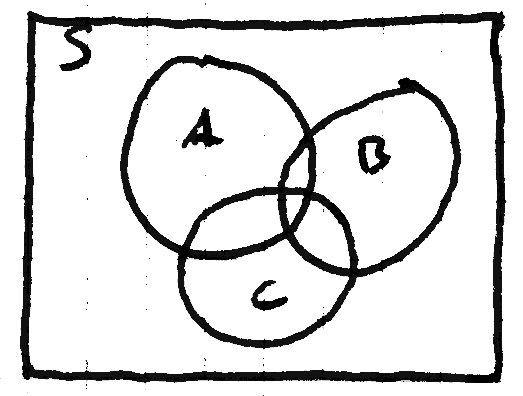
\includegraphics[width=.25\textwidth]{./Bilder/b03.jpg}
    % b01.jpg: 495x434 pixel, 72dpi, 17.46x15.31 cm, bb=0 0 495 434
  \end{figure}
  
  Gehe von einem Problem aus, bei es leicht ist zu zählen, welche Elemente aus dem Universum \(S\) die Eigenschaft \(A\) oder \(B\), \(A\) und \(B\), ... erfüllen; es aber schwer ist zu zählen, wie viele Elemente diese Eigenschaften nicht besitzen. Es ergibt sich jedoch der Zusammenhang
  \[
    | \overline{A \cup B \cup C} | = |S| - ( |A| + |B| + |C| ) + ( |A \cap B| + |A \cap C| + |B \cap C| ) + ( | A \cap B \cap C | )
  \]
  Sind \(N\) Objekte und eine Menge \(P = \{ P_1, ... P_n \}\) von Eigenschaften gegeben, bezeichnen wir für jedes \(S \subseteq P\) mit \(N(S)\) die Anzahl der Objekte, die (mindestens) die Eigenschaften in \(S\) erfüllen. Mit \(N(0)\) bezeichnen wir die Anzahl der Objekte, die keine der Eigenschaften erfüllen. Wir können oben skizzierte Formel dann verallgemeinern, es ergibt sich
  
  \begin{theorem}
    \(N(0) = \sum_{S \subseteq P} (-1)^{|S|} N(S) = N(\emptyset) + \sum_i N(P_i) + \sum_{i \leq j} N(P_i, P_j) + ...\).
  \end{theorem}
  
  \begin{proof}
    Elemente des Universums, die keine der Eigenschaften besitzen, werden auf beiden Seiten der Gleichung einmal gezählt. Betrachte nun die Elemente, die genau die Eigenschaften \(S = \{ P_{i_1}, ..., P_{i_s}\}\), \(|S| = s\). Diese werden genau in den \(N(S')\) mit \(S' \subseteq S\) gezählt. Daraus folgt, dass diese Objekte zur rechten Seite der Gleichung jeweils \( \sum_{S' \subseteq S} (-1)^{|S'|} = \sum_{i=0}^s \binom{s}{i} \cdot (-1)^i = (-1 + 1)^s = 0\) beitragen. Objekte, die mindestens eine Eigenschaft besitzen, werden also auf der rechten Seite nicht gezählt.
  \end{proof}


